\documentclass[../main_proj5.tex]{subfiles}

\graphicspath{{\subfix{Figures/}}}

\begin{document}

\section{Theory}\label{sec:p5_theory}


\subsection{The Schr\"{o}dinger equation and Borns rule}

Including time-dependencies the general formulation of the Schr\"odinger equation is 

\begin{equation}
\label{eq:p5_general_schrodinger}
    \text{i} \hbar \frac{d}{dt} \ket{\Psi} = \hat{H} \ket{\Psi} \quad ,
\end{equation}

\noindent where; $\text{i} = \sqrt{-1}$ is the imaginary unit, $\hbar$ is the reduced Planck constant defined by $\hbar:= h/2\pi$, $\hat{H}$ is the Hamiltonian operator and $\ket{\Psi}$ is the quantum state \cite{prosjekttbeskrivelse5}. 

$\ket{\Psi}$ represents the quantum state in general and without considering the specific basis for the physical space. For a non-relativistic particle in \textit{position space} with a position given by $\mathbf{r}$ the quantum state is represented by the complex-valued wave function $\Psi(\mathbf{r})= \bra{\mathbf{r}\ket{\Psi}}$ \cite{prosjekttbeskrivelse5}. Further, working in position-space yield the Hamiltonian as 

\begin{equation}
\label{eq:p5_hamiltonian}
    \hat{H} = - \frac{\hbar^{2}}{2m} \frac{\partial^{2}}{\partial\mathbf{r}^{2}} +V(\mathbf{r}) \quad,
\end{equation}

\noindent where $m$ is the particle mass and $V(\mathbf{r})$ represents a time-\textit{independent} external environment for the particle. 

In quantum mechanics each observable (e.g. position, momentum, energy etc) is associated with a linear Hermitian operator (see chapter 5 in \cite{townsend2010quantum} for details on implications). When the operators of different observables do not commute, that is, its commutator do not vanish an uncertainty relation is formed \cite{townsend2010quantum}. This is the case for the position operator $\mathbf{r}_{\operatorname{op}}$ and the momentum operator $p_{\mathbf{r}_{\operatorname{op}}}$ which yields the Heisenberg uncertainty relation 

\begin{equation}
\label{eq:p5_heisenberg_uncertainty}
    \Delta \mathbf{r} \Delta p_\mathbf{r} \geq \frac{\hbar}{2} .
\end{equation}

\noindent Here $\Delta$ indicates that there is some uncertainty attached to the measurement. The consequences is that we can not conduct a precise measurement of both the position and movement of the particle at the same time. This illustrates the need for Born's rule which postulates that a measurement of a quantum system yields the \textit{probability} of the given result, rather then some exact metric. For this study we use Born's rule to interpret the normalized squared value of the wave function as the probability density for where the particle is positioned in space. At a time $t$ the mathematical formulation becomes
\begin{equation}
\label{eq:p5_borns_rule_positionspace}
    p(\mathbf{r}; t) = |\Psi(\mathbf{r}, t)|^{2} = \Psi(\mathbf{r}, t)^* \Psi(\mathbf{r}, t) , 
\end{equation}

\noindent where $^*$ signifies taking the complex conjugate- To allow for this probabilistic interpretation of the wave function Born's rule also implies that probability must be conserved in the system. Further a normalization of the probability is also needed to interpret how different wave functions interact with the system \cite{townsend2010quantum}. Therefor we require 

\begin{equation}
\label{eq:p5_normalization_condition}
    \int\limits_{-\infty}^{\infty} p(\mathbf{r;} t)d\mathbf{r} = 1 .
\end{equation}


%The Hamiltonian is a linear Hermitian operator of energy where $- \frac{\hbar^{2}}{2m} \frac{\partial^{2}}{\partial\mathbf{r}^{2}}$ expresses the particles kinetic energy. This implies that we can formulate the equation as an eigenvalue equation for which the only possible results of measurements of energy are at the eigenvalues, i.e., we have discretized energy values \cite{townsend2010quantum}. 




% ===========================================================================
% Method
% ===========================================================================

\subsection{The scaled Schr\"odinger equation}

In this study, we examine a non-relativistic particle in a two-dimensional position-space. Substituting equation \eqref{eq:p5_hamiltonian} into equation \eqref{eq:p5_general_schrodinger} with $\mathbf{r}= [x, y]$ we get 


\begin{equation}
\label{eq:p5_full_schrodinger_p5}
    \text{i}\hbar \frac{\partial}{\partial t} \Psi = \\
    -\frac{\hbar}{2m}\left(\frac{\partial^{2}}{\partial x^{2}} + \frac{\partial^{2}}{\partial y^{2}}\right)\Psi + V(x,y)\Psi,
\end{equation}

\noindent where we have omitted the ''function-off`` notation for $\Psi(x,y,t)$. Assuming that dimensionful variables have been scaled away, \eqref{eq:p5_full_schrodinger_p5} can be simplified to 

\begin{equation}
\label{eq:p5_scaled_schrodinger_p5}
    \text{i}\frac{\partial u}{\partial t} =
    -\frac{\partial^{2}u}{\partial x^{2}} - \frac{\partial^{2} u}{\partial y^{2}} + v(x,y ) u,
\end{equation}

\noindent where all variables are dimensionless with $u(x,y,t)$ as some complex-valued scaled wave function \cite{prosjekttbeskrivelse5}. Using the notation from equation \eqref{eq:p5_scaled_schrodinger_p5} Born's rule become
\begin{equation}
    \label{eq:p5_scaled_borns_rule_positionspace}
    p(x,y;t) = |u(x,y,t)|^{2}.
\end{equation}

\noindent To solve this system with a propagating particle we will use the numerical Crank-Nicolson method in this study.


\subsection{Crank-Nicolson discretization}

In this study we will use a square potential with $x,y \in[0, 1]$. We will simulate over times $t\in[0, T]$ where $T$ will be varied between experiments (see Section \ref{sec:p5_implementation_experment design} for details). Further, we let $i$, $j$ and $n$ denote the index in the discretized $x, y$ and $t$ with $i,j = 0, 1, \dots, M-1$ and $n = 0, 1, N_t-1$ respectively. Consequently, the spatial resolution of the discretization is $h=\frac{1-0}{M-1}$ including the boundary points and the temporal resolution is $\Delta t = \frac{T-0}{N_t}$. For an arbitrary point in the spatio-temporal space the scaled wave function is denoted by 
\begin{equation}
\label{eq:p5_discretized_scaled_wavefunction}
u(x_i, y_j, t_n)=u(ih, jh, \Delta t):=u_{ij}^n ,    
\end{equation}

\noindent for which we introduce the matrix $U^{n}\in\mathbb{C}^{M\times M}$ to hold all values $u_{i,j}^{n}$. To constrain the problem we use Dirichlet boundary conditions implying $u_{ij}^{n} = 0$ for all $i,j =0 || M-1$. Similarly, the potential is denoted as 

\begin{equation}
    v(x_i, y_j) = v(ih,jh) = v_{ij} ,
\end{equation}

\noindent which we store in the matrix $V\in\mathbb{R}^{M\times M}$. 

The general form of the original Crank-Nicolson scheme for an equation of the form $\frac{\partial u}{\partial t} = F(x, y, t)$ is 

\begin{equation}
    \label{eq:p5_general_Crank_Nicolson}
    \left(\frac{\partial u}{\partial t} \right)_{ij}^n = 
    \frac{1}{2}\left[F_{ij}^{n+1} + F_{ij}^{n}\right] \quad, 
\end{equation}

\noindent where we have introduced the same short-hand notation for the derivatives and $F$ as that of $u(x,y,t) \to u_{ij}^n$ \cite{lecture_notes}. For equation \eqref{eq:p5_scaled_schrodinger_p5} the Crank-Nicolson formulation implies that 

\begin{equation}
    F(x,y,t) = -\frac{\partial^{2}u}{\partial x^{2}} - \frac{\partial^{2} u}{\partial y^{2}} + v(x,y ) u \quad.
\end{equation}

To discretize we use forward difference for the first-order partial derivatives and the general form for the second-order partial derivatives. Further, by using the approximate terms (i.e. omitting the terms; $\mathcal{O}(\Delta t)$ and $\mathcal{O}(h^{2})$) we show in Appendix \ref{app:p5_AppendixA_discretized schrodinger} that the scaled Schr\"odinger equation can be written as 

\begin{equation}
\label{eq:p5_discretized_schrodinger_crank_nicolson}
\begin{split}
    u_{ij}^{n+1} &  \\
    - r \left[u_{i+1,j}^{n+1} - 2u_{ij}^{n+1} + u_{i-1,j}^{n+1}\right] & \\
    - r \left[u_{i,j+1}^{n+1} - 2u_{ij}^{n+1} + u_{i,j-1}^{n+1}\right]&  \\
    + \frac{i \Delta t}{2} v_{ij} u_{ij}^{n+1} &=   u_{ij}^n \\
    & +r \left[u_{i+1,j}^n - 2u_{ij}^n + u_{i-1,j}^n\right]  \\
    & +  r \left[u_{i,j+1}^n - 2u_{ij}^n + u_{i,j-1}^n\right]  \\
    &  -  \frac{i \Delta t}{2} v_{ij} u_{ij}^n 
\end{split}, 
\end{equation}

\noindent where $r$ is a constant defined as $r := \frac{\text{i} \Delta t}{2 h^{2}}$. From this discretization we see that propagation forward in time implies a computational stencil using all four nearest neighbors in the discretized position space. 
 
In Appendix \ref{app:p5_AppendixA_matrix_vector} we show that we can re-write equation \eqref{eq:p5_discretized_schrodinger_crank_nicolson} as a matrix-vector equation on the form 

\begin{equation}
\label{eq:p5_general_matrix-vector-equation}    
    A \mathbf{u}^{n+1} = B \mathbf{u}^{n}.
\end{equation}

\noindent In this formulation the constants used to scale the significance of neighboring wave function values are store in $A$ which is a five-diagonal banded matrix in $\mathbb{C}^{N_{int}^{2}\times N_{int}^{2}}$. Similarly the right hand side constants are stored in $B$. Further, $\mathbf{u}^{n(+1)}$ are column vectors in $\mathbb{C}^{N_{int}^{2}}$ holding the vertically stacked internal points from the columns of the state matrix $U^{n(+1)}$. 

% ===========================================================================
% Implementation
% ===========================================================================

\subsection{initialization}

Since we are simulating a physical system we have to place the particle in some form of surroundings, here represented by the matrix $V$. Figure \ref{fig:two-slit_setup} show the two-slit setup which is used for most simulations. Black areas are walls where $v_{ij}$ is set to 10 \% of the maximum available in c++ doubles. White areas are set to 0.

\begin{figure}[h!]
    \centering
    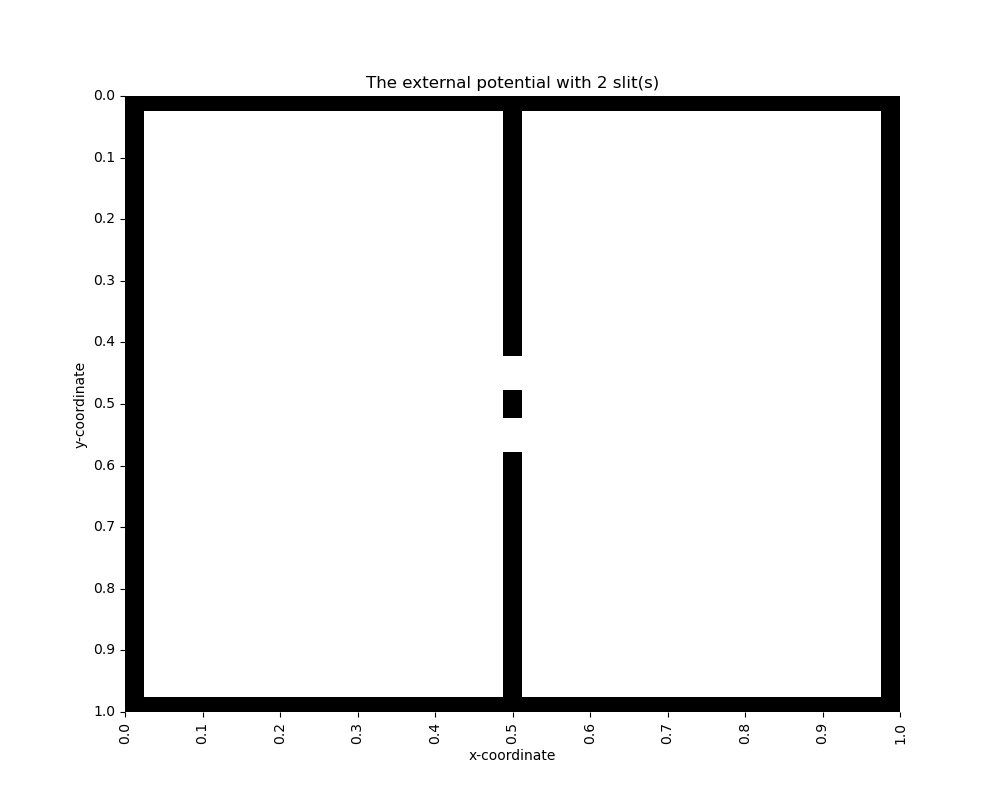
\includegraphics[width=0.9\linewidth]{Project 5/figures/2slits.png}
    \caption{The two slit external environment which the particle is placed in. Black areas are walls where $v_{ij}$ is set to 10 \% of the maximum available in c++ doubles. White areas are set to 0. }
    \label{fig:two-slit_setup}
\end{figure}

\noindent The initialization of $V$ will vary between the number of slits used in the simulation, however the center wall will always centered at $x=0.5$. Further, the slits will always be symmetric around $y=0.5$ with a slit aperture of $0.05$ and a separation segment of $0.05$.  

To simulate the propagation of a wave packet using equation \eqref{eq:p5_general_matrix-vector-equation} we need some initial values which we represent by $U^{0}$. In this study we initialize the wave packet using the Gaussian distibution 

\begin{equation}
\label{eq:p5_gaussian_wave}
    u(x,y, t=0) = e^{\left[ 
    - \frac{(x-x_c)^{2}}{2\sigma_x^{2}} - \frac{(y-y_c)^{2}}{2\sigma_y^{2}} +\text{i}(p_x x + p_y y)
    \right]},
\end{equation}

\noindent where $x_c, y_c$ are the mean of marginal distributions, therefor dictating the coordinate of the center of the initial wave function. $\sigma_x, \sigma_y$ is the standard deviation, signifying the initial width of the distributions and $p_x, p_y$ is the wave-packet momenta \cite{prosjekttbeskrivelse5}. To fulfill the boundary conditions we set $u_{ij}^{0} = 0$ for all $i, j$ where $\operatorname{abs}(v_{ij}) > 10^{-10}$, that is, when we are in a wall. 

To apply Born's rule we normalize $U^{0}$ by 
\begin{equation}
    U_{\operatorname{normalized}}^{0} = \frac{U^{0}}{N^{0}},
\end{equation}

\noindent where $N^{0}$ is the normalization factor estimated by
\begin{equation}
    N^{0} = \left(
    \sum\limits_{i,j} |u_{i,j}^{0}|^{2}
    \right)^{\frac{1}{2}} .
\end{equation}

\noindent $U_{\operatorname{normalized}}^{0}$ will now satisfy equation \eqref{eq:p5_normalization_condition} allowing us to interpret $p_{ij}^{0}$ as the probability at $t=0$ of a particle being in the area $h^{2}$ centered on $(ih, jh)$. Given numerical stability this will be true for all $n = 0, 1, ..., N_t$. Further, the normalized marginal distributions for one of the spatial dimensions, that is, $p(y| x=ih ; t=n)$ or $p(x|y=jh; t=n)$ is interpretable as a detection screen commonly used in interference experiments.

After initializing $V$ and $U$ we initialize the coefficient matrices $A$ and $B$. These are filled with the constants from equation \eqref{eq:p5_discretized_schrodinger_crank_nicolson} on five diagonals. Because of this, and their large size, they are stored as sparse matrices during simulation.

During the initialization we set multiple parameters; number of slits for $V$, position, width and momenta for $U$ and the discretization resolution which affects all. In Section \ref{sec:experimental_design} we present  details on which configurations are used for which experiments. 

\subsection{Solving the equation}



To solve equation \eqref{eq:p5_general_matrix-vector-equation} involves a two step approach; first we  calculate 
\begin{equation}
    \mathbf{b} = B \mathbf{u}^{n} ,
\end{equation}


\noindent that is, we take the matrix-vector product with the known $\mathbf{u}^n$ yielding $\mathbf{b}\in \mathbb{C}^{N_{int}^{2}}$. Next we solve 

\begin{equation}
    A \mathbf{u}^{n+1} =\mathbf{b} ,
\end{equation}

\noindent for $\mathbf{u}^{n+1}$ which implies performing and inverse of $A$. Since the coefficient matrices are very large inversion is not feasiable with computation of the determinate \cite{Linear_Algebra_and_its_Applications}. Rather we have to consider other direct methods such as Gaussian elimination and LU decompositions or indirect methods such as Jacobi's iterative method and Gauss-Seidel. The indirect methods are often preferred for large matrices since they are often less prone to round-off errors \cite{lecture_notes}. Further they only use non-zero elements for computation and can therefore work without keeping the whole matrix in memory. However these method's are not guarantied to converge to an exact solution. However, in this study we use the superLU implementation (LU decomposition for sparse matrices) from the armadillo c++ library (see \cite{liOverviewSuperLUAlgorithms2005} for details). This allows us to use the direct method also for large matrices. The advantage of the direct methods is that they \textit{can} converge to the exact solution as opposed to indirect methods. 

SuperLU build on the LU-decomposition where a square matrix $A$ is decomposed on the form 

\begin{equation}
    \label{eq:LU}
    A = LU, 
\end{equation}

\noindent which, for larger matrices, allows for a calculation of the inverse which is smaller then that of inverting $A$ directly. We expect a high order of numerical stability using this method.



\subsection{Experiment design} \label{sec:experimental_design}

To assess the numerical stability of the implementation we will assess if the requirement of \eqref{eq:p5_normalization_condition} is fulfilled through the whole simulation. We will run two simulations for this assessment with the spatial dimensions discretized with $h=0.005$ and a temporal discretization of $\Delta t = 2.5 * 10^{-5}$ over the simulation length $T=0.008$. The wave-packet ''settings`` for one simulation will be initialized with  $\mathbf{r}_c = (0.25, 0.50)$, $\mathbf{\sigma}=(0.05, \sigma_y)$, $\mathbf{p}=(200, 0)$. The two simulations are distinct in that the first will be performed with 0 slits, that is, only border-walls, and the second one will have a double slit wall. Further, we use a narrower wave packet in the first simulation with $\sigma_{y}=0.05$ as opposed to $\sigma_y=0.10$ in the second simulation. We will refer to these simulations as the numerical stability experiment.

Next we want to assess the behavior of the wave packet as it is propagated towards a double slit. To do this, we use the same values for $h$, $\Delta t$, $\mathbf{r}_c$, $\sigma_x$ and $\mathbf{p}$ as in the assessment of the numerical stability. We will however, reduce the simulation time to $T = 0.002$ and increase the with by setting $\sigma_y=0.20$. By varying the number of slits through the set $\{1, 2, 3\}$ we will also asses the probability of detecting a particle with a detector screen at $x=0.8$. This implies finding the marginal distribution $p(y|x=0.8 ;t=0.002)$. We will refer to these simulations as the slit experiment. 


\subsection{Tools}

All simulation code is written in c++ using the armadillo library for vector and matrix handling. Python is used for scripting the .cpp compilation using CMake and to plot during runtime. Some illustrations are also produced using jupyter notebooks and matplotlib, seaborn, cmocean and PIL. GDB has been used for debugging. 

I have used the copilot codeium (\href{https://codeium.com/}{https://codeium.com/}) to aid with c++ syntax and python plotting. However, I have not used it to develop any parts of the code unsupervised, all code structure is therefor created by me.

\end{document}
